\documentclass[pdftex, a4paper]{scrartcl}
%\documentclass[pdftex, a4paper]{scrreprt}
\usepackage{ngerman}
\usepackage[utf8]{inputenc}
\usepackage[T1]{fontenc}
%x\usepackage{parskip}
\usepackage{array}
\usepackage{natbib}
\usepackage{subfiles}
%\usepackage{filecontents}
 \usepackage{url}

\makeglossaries

\newacronym{cba}{CBA}{Click-and-Buy-Automat}
\newacronym{tcpip}{TCP/IP}{Transmission Control Protocol/Internet Protocol}
\newacronym{ehi}{EHI}{Handelsforschungsinstituts}
\newacronym{pin}{PIN}{Persönliche Identifikationsnummer}
\newacronym{uml}{UML}{Unified Modeling Language}
\newacronym{nfc}{NFC}{Near Field Communication}
\newacronym{ddos}{DDoS}{Distributed-Denial-of-Service}
\newacronym{nmap}{Nmap}{Network Mapper}
\newacronym{2fa}{2FA}{Zwei-Faktor-Authentisierung}
\newacronym{mfa}{MFA}{Multi-Faktor-Authentisierung}
\newacronym{bsi}{BSI}{Bundesamt für Sicherheit in der Informationstechnik}
\newacronym{ki}{KI}{Künstliche Intelligenz}
\newacronym{ai}{AI}{Artificial Intelligence}






\fancypagestyle{mylandscape}{
\fancyhf{} %Clears the header/footer
\fancyfoot{% Footer
\makebox[\textwidth][r]{% Right
  \rlap{\hspace{2cm}% Push out of margin by \footskip
    \smash{% Remove vertical height
      \raisebox{4.87in}{% Raise vertically
        \rotatebox{90}{\thepage}}}}}}% Rotate counter-clockwise
\renewcommand{\headrulewidth}{0pt}% No header rule
\renewcommand{\footrulewidth}{0pt}% No footer rule
}



\begin{document}
    \begin{titlepage}
    \vspace*{7cm}
    \begin{center}
        \Huge
        Vermeidung und Verhinderung von DoS und DDoS Angriffe\\
        \vspace{1cm}
        \large
        \vspace{2cm}
        %Bruno Macedo da Silva - Matrikelnummer xxxxxxxxx \\
        %Dominic Meier         - Matrikelnummer xxxxxxxxx
         \begin {table}[ht]
             \centering
             \begin{tabular}{c|c}
                 \textbf{Name} & \textbf{Matrikelnummer} \\
                 Bruno Macedo da Silva & xxxxxxxxx \\
                 Dominic Meier         & xxxxxxxxx \\
             \end{tabular}
         \end {table}
    \end{center}
    \normalsize
    \vfill
    Copyright (C) 2020 xxxxxxxxxxxxx.

    Bla bla bla bla bla bla bla bla bla bla bla bla bla bla bla bla bla. bla bla bla bla bla bla bla bla. 
    bla bla bla bla bla bla bla bla. bla bla bla bla bla bla bla bla. bla bla bla bla bla bla.bla bla.

    bla bla bla bla bla bla bla bla bla bla bla bla bla bla bla bla bla bla bla bla bla bla bla bla bla bla.
    bla bla bla bla bla bla bla bla bla bla bla bla bla bla bla bla bla bla bla bla bla bla bla bla.
    bla bla bla bla bla bla bla bla bla bla bla bla bla bla bla bla bla bla .


    bla bla bla bla bla bla bla bla bla bla bla bla bla bla bla bla bla bla.


\end{titlepage}
    \tableofcontents
    \newpage
    \listoffigures
   \clearpage
   \printglossary[type=acronym,title=Abkürzungsverzeichnis,toctitle=Abkürzungsverzeichnis]
	  \clearpage
    \section{Einführung}


Seit einigen Jahren entscheiden sich immer mehr Menschen Urlaub auf einem Campingplatz 
zu machen. Der Gedanke an Menschenmassen und Fallen für Touristen schreckt die Leute von
den typischen Touristenzielen ab. Zudem ist der Kontakt zu der Natur für viele ein wichtiger
Teil in einem Urlaub. In den letzten anderthalb Jahren stieg die Anzahl von Campinplatzbesuchern
rasant. Die Corona-Pandemie drängte die Leute dazu, Urlaubsmöglichkeiten zu suchen, bei denen
das Risiko von einer Infektion niedrig sei und wo genug Abstand gehalten werden könne. Da viele 
Hotels und andere Ferieneinrichtungen geschlossen waren, blieb vielen Leuten, besonders Familien,
nichts anderes übrig, als die Ferien etwas anders zu organisieren und gestalten.


\textbf{Hotels Gesellschaft}
\textbf{Click and Buy = Definition mit Footsnote}


Die traditionelle Idee von Campingplätzen, bei der Jugendliche oder Familien weit entfernt von der 
Gesellschaft sind, ist heute eine andere. Heute wollen Urlauber auf den Kontakt mit der Natur
möglichst nicht verzichten, wodurch Campingplätze immer voller werden. Aus diesem Grund wäre es
sinnvoll, die Möglichkeiten zur Grundversorgung zu erweitern, ohne direkt einen neuen Supermarkt
bauen zu müssen. In dieser Hinsicht kann die Einrichtung eines elektronischen Click-and-Buy-
Supermarktes, der mit einem Automaten zu vergleichen ist, eine wesentliche Rolle spielen, um 
einen Campingplatz und die Gegend drum herum zu modernisieren, die Möglichkleiten zur Grundversorgung 
zu erweitern und ihn attraktiver für Reisende zu machen.

Die Sicherheit der digitalen Zahlungsmethoden stellt eines des wichtigsten Punkte für die Entwicklung
eines solchen Systems dar. Vernachlässigungen in diesem Bereich führen zu unberechenbaren Vertrauensverlust 
seitens der potenziellen Nutzenden und zu finanziellen und moralischen Schäden der direkten
Stakeholder. Der folgende Artikel soll beschreiben, welche Schritte auf digitaler Sicherheitsebene 
eingeleitet werden müssen, um einen akzeptablen und funktionierenden Click-and-Buy-Automat errichten 
zu können. 

\textbf{Die Forschungsfrage am Ende der Einführung. Beenden dieses Kapitel mit der Frage.} 
\textbf{Frage als Ziel Formulierne}
\textbf{Erster Satz von Ziel = Frage --- um zu das zu machen. Um das zu machen, machen wir das das das}

\textbf{Fussnote krypto verfahren}


    \section{Forschungsziele}


In diesem Artikel soll ein Konzept für ein Click-and-Buy-Supermarkt direkt neben dem Campingplatz 
entwickelt werden. Solch ein Konzept kann dazu beitragen, dass Campingplätze und die Gegend
modernisiert werden und noch mehr Touristen angelockt werden. Bevor das Projekt jedoch umgesetzt 
werden kann, müssen noch wichtige Dinge beleuchtet werden. 


Um einen elektronischen Supermarkt zu entwickeln, müssen einige Voraussetzungen erfüllt werden.
Es sollte eine ausreichende Verfügbarkeit des Netzwerkzugangs gewährleistet werden, eine stabile 
Software, die den Qualitätsstandards entspricht, ein sicherer Umgang mit Kundendaten, der sich an 
spezifischen und internationalen Richtlinien orientiert, ein benutzerfreundliches System, das sich an 
verschiedenen Kundentypen, wie Alters- und Bildungsgruppe anpasst und letztlich ein kryptographisches
Verfahren für das bargeldlose Bezahlen, das die Vertraulichkeit sicherstellt.


Um die Verfügbarkeit des Netzwerkzugangs für den Click and Buy Automat zu gewährleisten, muss zum einen 
geprüft werden, ob die bereits vorhandenen Leitungen ausreichen, um solch ein Projekt umsetzen zu können.
Die Vernetzung soll so aufgebaut sein, dass es auch in remoten Regionen einwandfrei funktioniert. 
Die Software muss zudem so entwickelt werden, sodass diese eine geringe Ausfallquote aufweist, 
denn der Automat soll rund um die Uhr betriebsbereit sein, um das Ziel der Verfügbarkeit des
 Systems nicht zu verletzen \cite{refbook:SWIS}.


Zudem soll das System so entwickelt werden, sodass auch Digital Non-Natives, die Möglicheit
\cite{refart:QWDN} haben das System einfach bedienen zu können. Die Kunden sollten also nicht von 
Informationen überladen werden, sondern es sollte einfache Ein- und Ausgaben geben. Da sich besonderes
ältere Menschen für solch eine Urlaubsmöglichkeit entscheiden, spielt es für den Erfolg des Konzeptes 
eine entscheidene Rolle, dass auch sie mit dem Automaten umgehen können. Deshalb sollten die Bedürfnisse
und Einschränkungen dieser Altergruppe besonders berücksichtigt werden, um ihr Vertrauen zu gewinnen
\cite{refart:HLAU} und hauptsächlich gegen Social Engeneering Angriffe zu schützen. Die Auswahl der
Tests trägt dazu bei, dass die Zufriedenheit und die Akzeptanz gewährleistet wird, sodass jeder 
potenziellen Endnutzer das System bedienen kann \cite{refbook:IASE}.

Außerdem spielt die Sicherheit bei den bargeldlosen Zahlungsvorgängen eine große Rolle und sollte
deshalb höchste Priorität haben. Verschiedene aktuelle Beispiele von Cyberangriffe zeigen, dass der 
Umgang mit solchen Daten, kritisch zu sehen ist. Es wird oft von Situationen in den Medien berichtet,
bei denen Kunden ihr Geld verloren haben oder dessen personenbezogenen Daten missbraucht wurden. 
In seltenen Fällen sogar von der eigenen Regierung, weil das System nicht ausreichend gegen Angriffe 
entwicklet wurde. In dieser Hinsicht sollten bei der Entwicklung spezifische und klare Richtlinien 
berücksichtig werden, sodass der sichere Umgang mit personenbezogenen Daten gewährleistet ist 
\cite{refart:TRVR}. Um diese Vertraulichkeitsverletzung zu vermeiden, spielt die Konziperiung von 
sicheren bargeldlosen Zahlungsmethoden eine wesentliche Rolle in diesem Artikel. 

Da das gesamte Thema sehr umfangreich ist, hier wird hauptsächlich die folgende Frage behanldet: 
Wie kann sicheres bargeldloses Bezahlen in einem Click and Buy Automat gewährleistet werden?
    \section{Stand der Forschung}


Die zunehmende Tendenz in Deutschland von bargeldloser Bezahlung erfordert neuen Umgang mit den 
eigegebenen Daten. Eine Studie von 2009 der Deutschen Bundesbank zeigte den rasanten Anstieg von 
bargeldloser Bezahlung in der Bundesrepublik seit der Einführung von solchen Zahlungsmethoden 
\cite{refrep:DBCP}.

\begin{figure}[htb]
    \centering{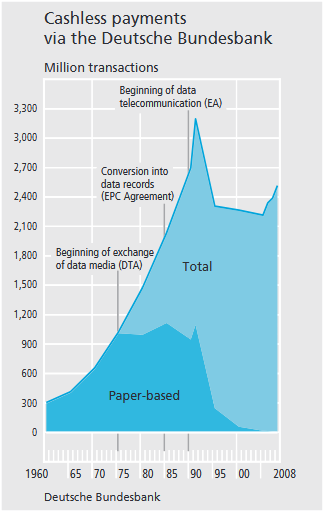
\includegraphics[width=5cm]{Bilder/refrep_DB.png}}
    \caption{Cashless payments via the Deutsche Bundesbank\\ (Bundesbank, 2009, S.52)}
    \label{fig:refrep_DB}
\end{figure}


Laut einer Statistik des Handelsforschungsinstituts EHI von 2019 \cite{refart:KSDL} bezahlen 48,6\% 
der deutschen ihre Waren mit Karte, wohingegen nur noch 46,9\% der deutschen den klassischen 
Weg mit Bargeld gehen. Auch das kontaklose Bezahlen, bei dem kleine Beträge nicht einmal mit einer 
PIN bestätigt werden müssen, nimmt immer weiter zu. Doch gerade bei dieser Variante ist es sehr einfach
im Namen eines anderen zu bezahlen, was eine Sicherheitsrisiko darstellt.


Immer wenn mit Karte bezahlt wird, gehen die Kunden davon aus, dass die Zahlungsabwicklung sicher ist. 
Wie sicher ist das bargeldlose Zahlen heutzutage wirklich? 


Aus diesem Grund ist Vertraulichkeit die erste und wichtigste Voraussetzung, dass ein solches System 
erfüllen muss, um neue potenzielle Kunden zu gewinnen. Unter diesem Begriff soll ein System nur auf 
autorisierte Informationen zugreifen \cite{refbook:SWIS}. In dieser Hinsicht ist die Entwicklung 
einer Click and Buy Maschine so zu konzipieren, dass sie einen sicheren Umgang mit den Kundendaten
anbietet. Diese Interaktion zwischen Kunde und systemkritischen Mechanismen wurde von 
\cite{refart:HARE} so dargestellt:

\vfill
\begin{figure}[htb]
    \centering{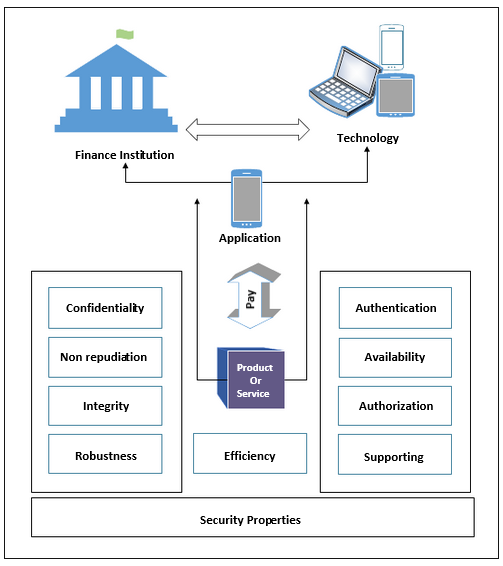
\includegraphics[width=5cm]{Bilder/refark_HARE.png}}
    \caption{Sicherheitseigenschaften von digitalen Zahlungsmethode (Hassan et al. 2020, S8)}
    \label{fig:refark_HARE}
\end{figure}
\vfill

Außerdem sollen die anderen Schutzziele der IT-Sicherheit: Integrität, Verfügbarkeit und
Authentizität auch berücksichtigt werden, sodass die Systemen einwandfrei und sicher funktionieren.
Eine Zahlungsmethode, bei der alle Vorraussetzungen erfüllt werden, kann in der Lage sein, das Vertrauen und 
die Akzeptanz von den Nutzenden zu bekommen \cite{refart:HARE}. 


\cite{inbook:MHNS} nennt solche Maschinen Cyber-Physical System (CPS), weil sie eine Interaktion zwischen 
Nutzer und einem oder vielen Systemen darstellt. In dieser Zusammenarbeit spielt der Datenaustausch 
eine wesentliche Rolle, besonders von der Seite der Nutzenden. Diese Technologie zielt eine günstigere 
Entwicklung, ohne die Sicherheit zu vernachlässigen. Diese Interaktion findet erfolgereich statt, 
wenn die genannten Sicherheitszielle erfüllt werden.


Da es um einen dynamischen Sektor geht, bei dem es sehr schnell zu Änderungen kommen kann, \cite{refip:NYRS} 
muss die Technologie stets weiterentwickelt und angepasst werden, um Vertraulichkeitsverlust seitens
der Kunden zu vermeiden. Da die Vertraulichkeit noch nicht zu 100 Prozent gewähleistet werden kann,
verweigern viele Kunden das bargeldlose Bezahlen.

\textbf{\textcolor{red}{Ab hier können wir dann versuchen, die Informatien aus den Artikeln zu nehmen, solche
die du hier hinzugefügt hast und solche, die ich dir am Fr schickte}}

\vspace{2cm}
\textbf{Ich würde diesen Satz in den nächsten Kapitel verwenden und erweitern mit unseren Recherchen, damit wird 
die Literatur rechtfertigen können}
Um das zu bewerkstelligen, ist der aktuelle technische Stand von entscheidener Bedeutung. 
Ausgehend von dieser Informationen muss das Glasfasernetz eventuell erweitert oder auch neu verlegt werden.
Denn das Ziel ist es, technisch gesehen auf dem neusten Stand zu sein, damit das Click and Buy System für die Zukunft abgesichert ist.
Außerdem wird durch den Ausbau des Glasfasernetzes die Region insgesamt deutlich attraktiver gemacht, was vielleicht auch Menschen dazu bringt
in diese Region zu ziehen. Denn jedem ist klar, dass ein guter Internetausbau essentiell ist, um vielleicht auch mal von zuhause aus zu arbeiten.
    \section{Stand der Technik}

Für die Bezahlungsmethoden werden hier zwei verschiedene Arten von Zahlungsverfahren analysiert und deren
Vorteile in Bezug auf Sicherheit und Härtungsmaßnahmen dargestellt: drahtlose Zahlung mit NFC und 
Smartcards.

\subsection{Drahtlose Verbindungen und Sicherheit bei Bezahlungen}

Viele digitale Zahlungen finden über NFC statt. Diese Technologie ermöglicht ein Zahlungs- und
Identifizierungsverfahren, indem ein passives Gerät oder auch Tag genannt mit einem aktiven Gerät,
auch Ermitter genannt, kommuniziert. In dieser Situation will das passive Gerät eine Autorisierung initiieren,
während das aktive Gerät für die Erlaubnis zuständig ist \cite{refart:NFNK}. 

\begin{figure}[H]
   \centering{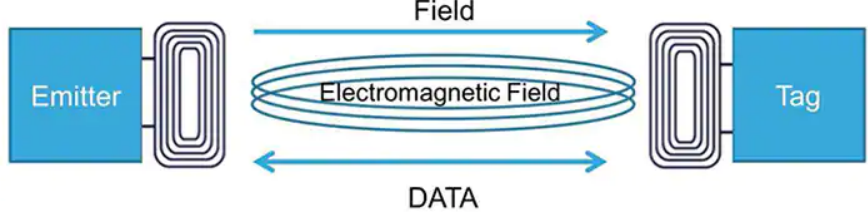
\includegraphics[width=8cm]{Bilder/refart_GPIN}}
   \caption{Teilnehmer der Kommunikation über NFC\\Quelle: Proehl, 2021}
   \label{fig:refart_GPIN}
\end{figure}
% \cite{refart:GPIN}

\subsubsection{Angriffsmöglichkeit auf NFC}

Da diese Technologie neu ist \cite{refip:NTAS}, sie existiert seit 2006, sind Schwachstellen 
und Härtungsmaßnahmen nicht in ihrer Vollständigkeit bekannt. Drahtlose Verbindungen sind auch für ihre 
Schattenseite bekannt \cite{refip:NYRS}. Maßnahmen zu entwickeln, die sich an verschiedene Systeme anpassen,
kosten Zeit und Investitionen von Banken und Sicherheitsfirmen. Für jeden möglichen Angriffe müssten 
Gegenmaßnahmen existieren, sodass das Schutzziel der Integrität\footnote{Es ist Subjekten nicht möglich, 
die zu schützenden Daten unatorisiert und unbemerkt zu manipulieren \cite{refbook:SWIS}.} nicht verletzt wird.

Bekannte Angriffe für kabellose Verbindungen können auch bei NFC verwendet werden\cite{refip:NYRS}, wie die
Erstellung und das Hinzufügen von Dateien in einem Opfersystem mit umfangreichen Privilegien; die Konzipierung
von schwachen digitalen Zertifikaten oder auch die Verwendung von Reverse Engineering\footnote{Reverse
Engineering ist ein Prozess von der Identifzierung von Bestandteilen eines Systems und von die Wiederherstellung 
dieser in einem anderen Format \cite{refart:CHRE}. Im Bereich der Cyber-Security wird Reverse-Engineering 
verwendent, um Schwachstellen von Systemen zu entedecken, sodass diese gegen Hardware und Software ausgenutzt
werden können \cite{refip:CMBM}.}. \cite{refart:ALSI} hebt andere Schwachstellen hervor: 
\textit{Eavesdropping}\footnote{Eavesdropping ist das unauthorisierte Mithören von einer Kummunikation 
\cite{refbook:SWIS}.} je nachdem, wie viele Ressourcen investiert werden, kann ein Angreifer in der 
Lage sein, der Kommunikation zu lauschen; \textit{Denial-of-Service}\footnote{Bei solchen Angriffen wird die
Verfügbarkeit des Dienstes verletzt, sodass die Kommunikation nicht mehr einwandfrei stattfinden kann 
\cite{refbook:SWIS}.}, um die Authentifizierung und Verfügbarkeit der Kommunikation zu beeinträchtigen.


\subsubsection{Gegenmaßnahmen für die Härtung von drahtlose Verbindung}

Um die Risiken bei der Verwendung von NFC zu abzuschwächen, schlägt \cite{refip:NYRS} einige Sicherheitsmechanismen vor, 
die sich eher auf allgemeine drahtlose Verbindungen beziehen und die auch für NFC verwendet werden können: Nutzung von modernen 
kryptographischen Standards für die Validierung von Zertifikaten; Verwendung von Zwei-Faktor- Authentifizierung; Erstellung
von schwer zu erratenden Passwörtern; Registrierung von authorisierten Geräten; Einsetzung von künstlicher Intelligenz 
(KI) für die Detektion von abweichendem Verhalten; Kontrolle gegen Social Engineering \footnote{Beim Social Engineering
nutzt der Täter den ``Faktor Mensch'' als vermeintlich schwächstes Glied der Sicherheitskette aus, um seine kriminelle
Absicht zu verwirklichen.\cite{booklet:BSSE}}

Kredit- und EC-Karten sollen auch als Zahlungsmittel bei unserem Click-and-Buy-Automat akzeptiert werden. 
In Bezug auf diese Zahlungsmittel, wird die Sicherheit im folgenden untersucht.

\subsection{Anwendung von Smartcards und sicheres Bezahlen}
Smartcards sind heutzutage stark verbreitet für eine Zahlungsabwicklung und auch für die Identifizierung.
Viele Ausweise, wie der Reisepass und die Krankenkassenkarte, verwenden diese Technologie zur Authentifizierung
des Nutzenden. Im folgenden ist ein Beispiel von einer Smartcard für eine zahlende Karte zu sehen: 

\begin{figure}[H]
   \centering{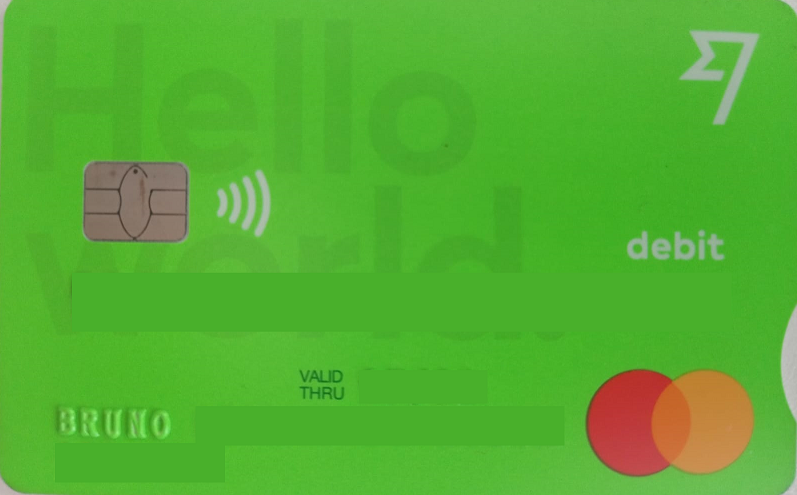
\includegraphics[width=4cm]{Bilder/eigenes_Bild_Karte.png}}
   \caption{Eine Smartcard und deren eingebetete Mikrochip\\Quelle: eigene Darstellung}
   \label{fig:eigenes_Bild}
\end{figure}

Die Smartcard wurde vor mehr als 40 Jahren erfunden und ihr Ziel ist die Sicherheit von Kartenzahlungen und 
allgemeine Authentifizierungsverfahren zu erhöhen \cite{refip:JFSB}. Sie unterscheiden sich von traditionelen 
Magnetstreifenkarten, weil sie verschiedene Authentifizierungsmethoden ermöglichen auch ohne eine direkte 
Verbindung zur Bank \cite{refbook:ATMS}. Im folgenden wird der Authentifizierungsprozess einer Smartcard 
\ref{fig:refbook_ATMS} dargestellt. 

\begin{figure}[H]
    \centering{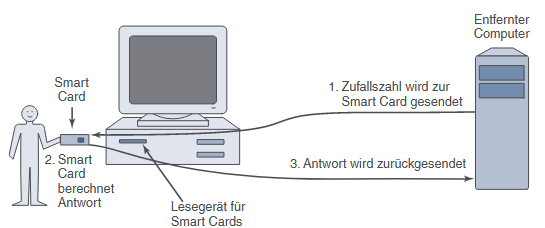
\includegraphics[width=6cm]{Bilder/refbook_ATMS.png}}
   \caption{Authentifizierungsprozess von Smartcards\\Quelle: Tanenbaum, 2009, S.755}
   \label{fig:refbook_ATMS}
\end{figure}

Die meisten Angriffe bei Smartcards geschehen laut \cite{refmas:ASSS} auf Hardwareebene. Er beschreibt folgende 
Techniken für Angriffe: Protokollanalyse, bei schwacher Konzipierung oder mangelnder Verschlüsselung ermöglichen Zugang 
zum Klartext; Hardware Reverse Engineering: Verständnis über die Algorithmen oder Extrahieren des Schlüssels


\subsubsection{Angriffsmöglichkeit auf Smartcards}
Smartcards sind auf Hardwareebene extrem sicher. \cite{refmas:ASSS} bezeichnet sie auch als ein in Hardware gegossener
Tresor für Informationen. Wenn eine Smartcard für das Bezahlen verwendet wird, ist kein Backend-System nötig,
denn alle wichtigen Informationen wie das Guthaben sind direkt auf der Karte gespeichert. Aus diesem Grund können
keine Daten abgefangen werden, die auf dem Weg vom Lesegerät zum Backend-System sind, was den Bezahlprozess
deutlich sicherer macht \cite{refbook:WRHC}. Zudem muss jede Kommunikation vom Lesegerät initiiert werden, 
die Karte selber startet also keine Kommunikation. Da die wichtigsten Daten direkt auf der Karte gespeichert sind,
muss ein Angriff auf die Hardware initiiert werden, um an relevante Informationen zu gelangen. Eine weitere 
Möglichkeit wäre, die Schwachstellen eines bestimmten Protokolls, das für die Kommunikation verwendet wird auszunutzen.

\subsubsection{Gegenmaßnahmen für die Härtung von Smartcards}
Um einen Angriff auf die Hardware möglichst zu vermeiden, ist es sinnvoll den Chip nicht rekonstruierbar zu machen,
d.h. dass keine Standardzellen oder ähnliches verwendet werden. Zusätzlich spielt die Verschlüsselung 
der Daten eine große Rolle und erhöht die Sicherheit enorm \cite{refst:ARES}. Außerdem können Mechanismen in 
die Smartcard eingebaut werden, die permanent die Spannung oder Frequenz überprüfen und sobald etwas
nicht dem Normalzustand entspricht, wird der Chip ausgeschaltet, sodass kein Lesegerät mit der 
Karte kommunizieren kann. Letztlich ist es wichtig, dass jede Karte individuell ist, sodass ein 
erfolgreicher Angriff kein Sicherheitsrisiko für andere Karten darstellt \cite{refmas:ASSS}. 
Dazu wären asymmetrische Verschlüsselungsverfahren sinnvoller als symmetrische, da jede Karte bei
asymmetrischer Verschlüsselung einen öffentlichen und privaten Schlüssel hat und somit alle einen unterschiedlichen
Schlüssel haben.


%- Smartcards sind auf der Hardwareebene extrem sicher. \cite{refmas:ASSS}  bezeichent Smartcards auch als 
%  ein in Hrdware gegossener Tresor für Informationen. 
%- das Guthaben oder der Verfügungsrahmen wird direkt auf der Karte gespeichert, sodass der ganze Prozess nicht über ein Backend-System laufen muss
%- die Komunikation wird immer vom Leser initiiert, die Karte reagiert nur
%- Angriffe richten sich direkt gegen die Hardware, nicht etwa Socail Engineering 
%- Analyse von übertragenen Daten --> Rückschlüsse auf Schwachstellen vom verwendeten Protokoll
%
%Gegenmaßnahmen:
%- damit der Chip nicht rekonstruierbar ist, sollte dieser möglichst Komplex sein, keine Standardzellen oder ähnliches einbauen
%- Zusätzlich lassen sich die Inhalte von Bussen und Speichern bereits auf Hardwareebene
%  durch Scrambling, das heißt das Vertauschen von Adressen, oder durch Verschlüsselung
%  der Daten schützen [2, S.540f][2, S.544f]. Schutzschichten, die den gesamten Chip umgeben
%  und von diesem permanent auf ihre Unversehrtheit geprüft werden, bilden eine weitere
%  Barriere die interne Funktionsweise zu analysieren [2, S.539f]. Andere Sensoren, etwa
%  zur Überwachung von Spannung oder Frequenz, können den Chip abschalten, sobald
%  diese einen Betrieb außerhalb der zulässigen Spezifikationen und damit einen möglichen
%  Angriff erkennen
%- Seitenkanal Angriffe können zum Beispiel durch immer gleich bleibenden Stromverbrauch verhindert werden
%- Grundvoraussetzung für ein sicheres System ist eine Authentifizierung der jeweiligen
%  Gegenstelle bei der Kommunikation, da nur so sicher gestellt werden kann, dass es sich
%  beim Kommunikationspartner nicht um einen Angreifer handelt [2, S.571]. Obwohl es
%  auch möglich ist, allein die Integrität übertragener Daten zu schützen, werden diese
%  oftmals zusätzlich verschlüsselt, sodass auch die Vertraulichkeit gewährleistet ist [2, S.570].
%  Alle für derartige kryptografische Operationen eingesetzten Algorithmen sollten öffentlich
%  bekannt und untersucht sein, um Sicherheitslücken soweit wie möglich auszuschließen [30,
%  S.9].
%  Bei der Implementierung der Algorithmen ist darauf zu achten, dass ein konstantes
%  Zeitverhalten gewährleistet wird, das heißt unabhängig von den Eingabedaten die gleiche
%  Ausführungszeit benötigt wird, um so darauf basierende Seitenkanalattacken zu unterbin-
%  den [2, S.560f]. Zufallszahlen, die unter anderem bei der Authentifizierung eine wichtige
%  Rolle spielen, sind auf kryptografisch sichere Weise zu erzeugen
%- Auf organisatorischer Ebene ist es wichtig, die Verwendung von kartenindividuellem
%  Schlüsselmaterial sicherzustellen, um zu verhindern, dass ein erfolgreicher Angriff auf
%  eine Karte auch andere Karten unmittelbar gefährdet. Dies geschieht entweder durch den
%  Einsatz asymmetrischer Kryptografie, bei der für jede Karte eigenes Schlüsselmaterial
%  generiert und von einer zentralen Instanz signiert wird, oder durch die so genannte
%  Key Diversification bei Verwendung symmetrischer Kryptografie. Hierbei wird unter
%  Einsatz einer Einwegfunktion ein kartenindividueller Schlüssel von einem Hauptschlüssel
%  abgeleitet und nur der abgeleitete Schlüssel auf der Karte gespeichert [30, S.22].
%  Sollte es zu einem Verlust oder einem erfolgreichen Angriff auf eine Karte kommen,
%  muss es möglich sein, diese Karte (genauer: ihr Schlüsselmaterial) im System zu sperren,
%  indem entsprechende Sperrlisten gepflegt werden [2, S.572]. Dass eine Karte angegriffen
%  und beispielsweise geklont wurde, lässt sich durch das Erstellen von Logeinträgen für
%  jede Verwendung und deren Überprüfung auf Unregelmäßigkeiten erkennen

\subsection{Fazit}

NFC ist eine Technologie die viele Vorteile bietet. Sie ermöglicht in nur einem Gerät die Anwendung verschiedener
Aktivitäten, wie Zahlung, Identifizierung und Authentifizierung, ohne dass ein Nutzer unterschiedliche Karten bei
sich haben muss. Die Nachteile beziehen sich auf die Neuigkeit dieser Technologie, die mehr Forschung verlangt, 
damit deren Schwachstellen weiter erforscht werden \cite{refart:ALSI}.  Die Technologie der Smartcards ist bereits
breit erforscht, sodass sowohl Schwachstellen, als auch Härtungsmaßnahmen bekannt sind. Die Akzeptanz und die 
Verwendung von Smartcards sind auch größer, da besonders Non-Natives eher auf Smartcards zurückgreifen.

Aus den obigen genannten Gründen können wir sagen, dass Smartcards der bessere Einsatz für einen Click-and-Buy-Automat
neben einem Campingplatz wäre, solange die Technologie von NFC noch nicht so weit erforscht ist und in der 
Gesellschaft nicht so etabliert ist.

    \section{Forschungsplann}


Keine Ahnung.


Grafische Darstellung des Forschungsvorhabens 

Methoden der Datensammlung ==> Besuch einigen Firmen


Methoden der Datendokumentation  ==> Aufnahme


Methoden der Datenauswertung ==> Vergleich der Daten der Firma (Anzahl Mitarbeiter, Anzahl Server/Pc, Seit wann benutzt es)


Anhang (Fragenkatalog) ==> Seitwann benutzt, was war vorher, was ist jetzt leichter/schwieriger, Kosten
    \section{Praktische Relevanz}

Die Entwicklung jedes Systems setzt die Akzeptanz von den Stakeholdern\footnote{Eine Person oder Gruppe, die Interesse für das Projekt 
haben oder auch die Beauftragter \cite{refip:HSSI}.} voraus. Um dieses Ziel zu erreichen, müssen einige Schritte befolgt
werden: Welche Wünsche haben die Stakeholder?; Hervorhebung der Anforderungen des zu entwicklendes Systems;
Tests des zu gestalteten Produkts; Implementierung des Systems oder der Anwendung; Weiterentwicklung des
Systems \cite{refbook:RECR}. Alle diese Schritte ermöglichen die Erzeugung eines potenziellen akzeptierten 
Systems, das von Kunden genutzt werden kann.

Relevent für Kunde weil
Firma weil
IT weil
Sozial weil


Diese geplante wissenschaftliche Arbeit soll vorallem Menschen nutzen, die in eher abgelegenen Orten wohnen und somit 
meistens von großen Supermarktketten vernachlässigt werden. Da der Automat 24 Stunden und 7 Tage in der Woche 
offen sein soll, können potenzielle Kunden auch mitten in der Nacht oder am Sonntag ihre Einkauf am \acrfull{cba} tätigen,
ohne für die überteuerten Preise von der Tankstelle bezahlen zu müssen. 

%Diese geplante wissenschaftliche Arbeit soll einen möglichst großen Nutzen haben und zudem sollen auch viele von dem geplanten 
%Projekt profitieren. Zum einen hat der \acrfull{cba} an sich schon einen riesen Nutzen, denn dieser wertet eine Region, in der
%dieser Automat steht extrem auf. Dieser Autoamt soll 24 Stunden und 7 Tage in der Woche offen sein. Das heißt, auch wenn beim
%normalen Einkauf im Supermarkt ein Artikel vergessen wurde, kann der Kunde diesen inm \acrfull{cba} auch mitten in der Nacht 
%oder am Sonntag kaufen, ohne die überteuerten Preise von der Tankstelle bezahlen zu müssen. 

Dadurch, dass der Automat rund um die Uhr funktioniert, ist es auch für die Lieferanten einfacher einen Termin für die Auslieferung 
der Waren zu finden. Denn es ist im Prinzip egal, wann die Ware eintrifft. Die Hauptsache ist, dass die Waren im \acrfull{cba}
möglichst immer verfügbar sind. 

Der eigentlich wichtigste Punkt ist die Sicherheit beim Bezahlvorgang, bei der es in der geplanten wissenschaftlichen Arbeit 
hauptsächlich geht. Das Ziel von der Entwicklung eines sicheren Zahlungsverfahren ist, dass die Kunden sich also keine Sorgen 
um die Sicherheit bei bargeldloser Bezahlung machen müssen, da die Methoden für die Bezahlung auf dem neusten technischen Stand sind.

Die Akzeptanz, die durch ein solches Verfahren entsteht, kann sogar auch dazu beitragen, Digital Non-Natives als potenzielle
Kunden zu gewinnen. Außerdem kann dieses Projekt andere Firmem dazu bringen, mehr in die Forschung für die Sicherheit bei
bargeldloser Bezahlung zu investieren.

%Aus unserer Sicht wäre es natürlich toll wenn wir durch den \acrfull{cba} auch Digital Non-Natives an das Thema der 
%bargeldlosen Zahlungsmethoden ranzuführen und somit alle Bezahlvorgänge zu vereinfachen.
%Außerdem werden vielleicht einige Firmen auf das Projekt aufmerksam und stecken noch mehr Zeit und Geld in die Forschung
%für die Sicherheit bei bargeldloser Bezahlung.
    \nocite{*}
    \bibliography{refart,refbook,refmisc,refunesed}
    \bibliographystyle{apalike}
        
\end{document}